\documentclass[../main.tex]{subfiles}

\begin{document}

\begin{titlepage}
%\AddToShipoutPicture*{\BackgroundIm}

   \begin{center}
       \vspace{-3cm}

       \Large{\textbf{\mytitle}}
       \vspace{0.2cm}
       %\vspace{0.5cm}

       \large{
    \begin{tikzpicture}
    \node[fill=white, fill opacity=1]{\textbf{\penname}}
    \end{tikzpicture}
    \vspace{0.2cm}

    {
    \begin{tikzpicture}
    \node[fill=white, fill opacity=1]{\textbf{Supervisor:}}
    \end{tikzpicture}
    %\vspace{-0.235cm}

    \begin{tikzpicture}
    \node[fill=white, fill opacity=1]{\textbf{Dr.~Dan Jones}}
    \end{tikzpicture}
    %\vspace{-0.235cm}


    \begin{tikzpicture}
    \node[fill=white, fill opacity=1]{\textbf{British Antarctic Survey}}
    \end{tikzpicture}
    }

    %\textbf{\supervisor}
    \vspace{0.5cm}

    \begin{tikzpicture}
    \node[fill=white,fill opacity=1]{\normalsize{\today}}
    \end{tikzpicture}
        }

       %\quickwordcount{main.tex}
       %\detailtexcount{main}
\vspace{3cm}

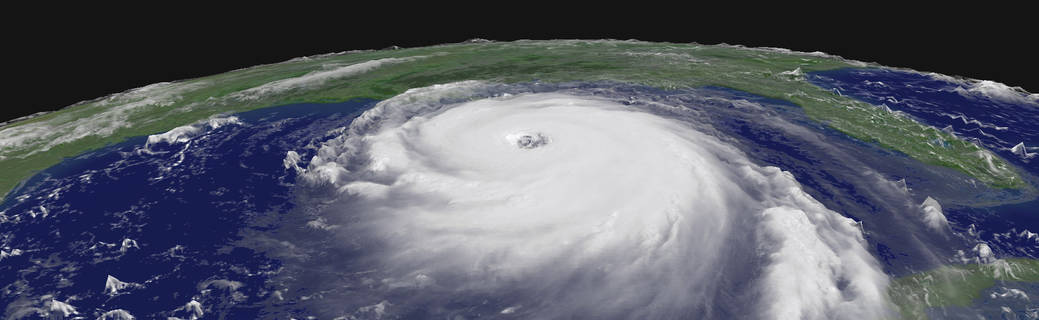
\includegraphics[width=\linewidth]{images/NASA-KATRINA-SIDEON.jpg}

%\textit{Image source: NASA}

   \vspace{3cm}
       \normalsize{
    \begin{tikzpicture}
    \node[fill=white,fill opacity=1]{A thesis submitted for the partial fulfilment of the
     }
    \end{tikzpicture}

    \begin{tikzpicture}
    \node[fill=white,fill opacity=1]{ degree requirements for Master of Natural Sciences.}
    \end{tikzpicture}
        }

       \vspace{0.4cm}


           \begin{tikzpicture}
    \node[fill=white,fill opacity=1] (a) {\large{
       \words~words}}
    \end{tikzpicture}
       \vspace{0.3cm}


       
\includegraphics[width=0.1\linewidth]{images/logos/UC.png}
       \vspace{0.8cm}
       % Cavendish Laboratory\\
       % University of Cambridge\\
   \end{center}
\end{titlepage}

\newpage
    \addtocontents{toc}{\protect\thispagestyle{empty}}
%\twocolumn[
  %\begin{@twocolumnfalse}
  {
  \vspace{-50pt}
%  \paragraph{Cover matter:}
  %An image from Nullschool.net on 28/10/19. Sea surface
  %temperature provides the colormap, and ocean currents provide the stripes.
%  \paragraph{Originality:} This is all my own original work
%                           unless otherwise highlighted.
  }

  \tableofcontents

%  \end{@twocolumnfalse}
  \paragraph{Length compliance:}

  /limit \\
  Abstract:  \abwords/500 words. \\
  Main body: \words/5000 words, \pages/30 pages.\\


  %There are few words to play with
 %and so much of the basic theory is placed in the appendix
 %(§~\ref{sec:ref-theory}) to this document.

 \begin{table}[ht]
\resizebox{\columnwidth}{!}{%
\begin{tabular}{l L{7.5cm}}

\hline \hline
\textbf{Term} & \textbf{Definition}\\
\hline
Bathymetry & Depth of the ocean (relative to geoid)\\
Isobath & Bathymetry contour \\
Inundation & The flooding of the land \\
Barotropic & Fluid density is only a function of pressure\\
Baroclinic & Fluid density is \textbf{not} only a function of pressure \\
\hline \hline
\end{tabular}
}
\caption*{Table: Assumed oceanographic terms in this thesis,
that would not
be defined in a paper. }
\label{tab:oceanographic}
\end{table}

 Hazard is defined as,
 \begin{equation*}
 \mathrm{Hazard}\equiv \int_{\mathcal{S}} \int \mathrm{risk}(E, S)  \cdot \mathrm{harm}(E, S)\; dE\; dS,
 \end{equation*}
 where risk is the probability of an extreme event, level $E$,
 and harm is the amount of damage at that $E$, and $S$ is the position
 in the region $\mathcal{S}$.
  \thispagestyle{empty}
%]

\newpage
\end{document}
